
\documentclass{article}
%%%%%%%%%%%%%
% Loads packages
%%%%%%%%%%%%%
\usepackage[table]{xcolor}
\usepackage[utf8]{inputenc}
\usepackage[colorlinks=true,linkcolor=blue]{hyperref}
\usepackage{geometry} %package needed to set margins
\usepackage{fancyhdr}
\usepackage{graphicx}
\usepackage{amsmath}
\usepackage{amsthm}
\usepackage{mdframed}
\usepackage{tikz}
\usepackage{amsfonts}
\pagestyle{fancy}
\fancyhf{}
\chead{\textbf{Homework 1}}
\lhead{Math 213, Fall 2024}
%%%%%%%%%%%%%
% Sets margins
%%%%%%%%%%%%%
\newgeometry{left=1.5in,right=1in,top=1in,bottom=1in}
\setlength\headsep{3pt}
%%%%%%%%%%%%%
% Creates problem and solution environments
%%%%%%%%%%%%%
% Solution Environment
\newenvironment{solution}{\begin{proof}[Solution]}{\end{proof}}
% Problem Environment
\newenvironment{problem}[1]
{\begin{mdframed}[default]
\textbf{Problem #1:}
}
{\end{mdframed}
}
%%%%%%%%%%%
% Custom Commands
%%%%%%%%%%%
\newcommand{\gOne}{\cellcolor{green!50!white} 1}
\newcommand{\rZero}{\cellcolor{red!50!white} 0}
\begin{document}
\textbf{Due Sunday, September 1st at 11:59pm}
\begin{problem}{\S 2.1: 10(a,c,e,g)}
Determine whether the following statements are true or false.
\begin{enumerate}
\item[(a)] $\emptyset \in \{ \emptyset \}$ 
\item[(c)] $\{ \emptyset \} \in \{ \emptyset \}$ 
\item[(e)] $\{ \emptyset \} \subset \{ \emptyset, \{ \emptyset \} \}$ 
\item[(g)] $\{ \{ \emptyset \} \} \subset \{ \{ \emptyset \}, \{ \emptyset \} \}$ 
\end{enumerate}
\begin{solution}{\S2.1:10(a,c,e,g)}
    \begin{enumerate}
\item[(a)]True
\item[(c)]False
\item[(e)]True
\item[(g)]False
    \end{enumerate}
\end{solution}
\end{problem}
\begin{problem}{\S 2.1: 16}
Use a Venn diagram to illustrate the relationships $A \subset B$ and $A \subset C$.

\end{problem}
\begin{figure}[h]
    \centering
    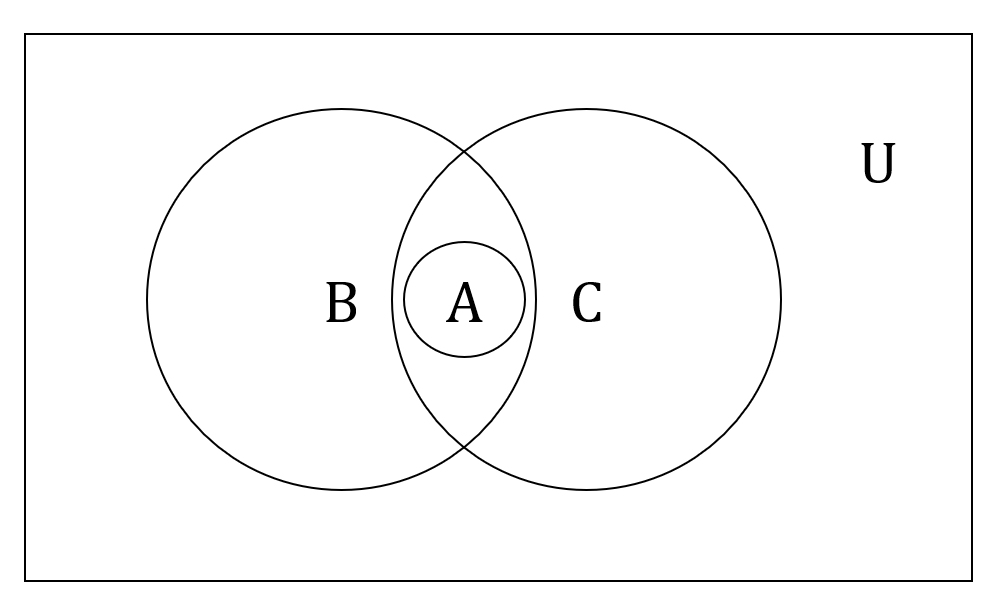
\includegraphics[width=0.35\linewidth]{Venen.png}
        \caption{Venn Diagram 2.1:16}
    \label{fig:enter-label}
\end{figure}

\begin{problem}{\S 2.1: 20}
What is the cardinality of each of the following sets?
\begin{enumerate}
\item[(a)] $\emptyset$ 
\item[(b)] $\{ \emptyset \}$ 
\item[(c)] $\{ \emptyset, \{ \emptyset \} \}$ 
\item[(d)] $\{ \emptyset, \{ \emptyset \}, \{ \emptyset, \{ \emptyset \} \} \}$ 
\end{enumerate}
\begin{solution}{\S2.1:10}
    \begin{enumerate}
\item[(a)]0
\item[(b)]1
\item[(c)]2
\item[(d)]3
    \end{enumerate}
\end{solution}
\end{problem}
\newpage
\begin{problem}{\S 2.1: 26}
Show that if $A \subseteq C$ and $B \subseteq D$, then $A \times B \subseteq C \times D.$\newline
Let $A$ is a set with $n$ items

Proof:

By the definition of Cartesian product $A \times B = \{(a,b)|a \in A \land b \in B\}$,
Since $A \subseteq C$ and $B \subseteq D$, $\forall a$, $a \in C$; $\forall b$, $b \in D$.
Define a set ${(a,b)|a\in C \land b \in D}$, by the definition of Cartesian product,
$\{(a,b)|a\in C \land b \in D\}=C \times D$.

\end{problem}
\begin{problem}{\S 2.1: 32(a,c)}
Let $A = \{ a, b, c \}$, $B = \{ x, y \}$, and $C = \{ 0, 1 \}$. Find the following
Cartesian products.
\begin{enumerate}
\item[(a)] $A \times B \times C$ 

\item[(c)] $C \times A \times B$\newline

Solution(a):

$A \times B \times C=\{(a,x,0),(a,y,0),(b,x,0),(b,y,0),(c,x,0),(c,y,0),$\newline
$(a,x,1),(a,y,1),(b,x,1),(b,y,1),(c,x,1),(c,y,1)\}$


Solution(c):

$C \times A \times B=\{(0,a,x),(0,b,x),(0,c,x),(1,a,x),(1,b,x),(1,c,x),$\newline 
$(0,a,y),(0,b,y),(0,c,y),(1,a,y),(1,b,y),(1,c,y)\}$


\end{enumerate}
\end{problem}
\begin{problem}{\S 2.2: 4}
Let $A = \{ a, b, c, d, e \}$ and $B = \{ a, b, c, d, e, f, g, h \}$. Find:
\begin{enumerate}
\item[(a)] $A \cup B$.
\item[(b)] $A \cap B$.
\item[(c)] $A - B$.
\item[(d)] $B - A$.\newline\newline
Solution:
\item[(a)] $A \cup B=\{a,b,c,d,e,f,g,h\}$.
\item[(b)] $A \cap B=\{a,b,c,d,e\}$.
\item[(c)] $A - B=\emptyset$.
\item[(d)] $B - A=\{f,g,h\}$.
\end{enumerate}


\end{problem}
\begin{problem}{\S 2.2: 14}
Find the sets $A$ and $B$ if $A - B = \{ 1, 5, 7, 8 \}$, $B-A = \{ 2, 10 \}$, and
$A \cap B = \{ 3, 6, 9 \}$.\newline
$A-B=\{1,5,7,8\}$means that elements:$\{1,5,7,8\}\in A $,$\{1,5,7,8\} \notin B$.\newline
$B-A=\{2,10\}$means that elements:$\{2,10\}\in B $,$\{2,10\} \notin A$.\newline
$A \cap B$means that elements$\{3,6,9\} \in A$and$B$\newline
so\newline$A=\{1,3,5,6,7,8,9\}$\newline$B=\{2,3,6,9,10\}$
\end{problem}
\begin{problem}{\S 2.2: 15}
Prove the second De Morgan law in Table 1 by showing that if $A$ and $B$ are sets,
then $\overline{A \cup B} = \overline{A} \cap \overline{B}$ (a) showing each side
is a subset of the other side and (b) by using a membership table.\newline

Proof:

\item[(a)] Showing each side is a subset of the other side.

To prove the equation, we prove by each side are the subset of the other side.
Suppose $x \in \overline{A \cup B}$, by the definition of complement, $x \notin A \cup B$.
By definition of union, we can see $\neg(x \in A \lor x \in B)$ is true.

By applying De Morgan Law, we get $\neg(x \in A) \land \neg(x \in B)$. 
Use definition of negation, we get $x \notin A \land x \notin B$,
By definition of complement, we get $x \in \overline{A} \land x \in \overline{B}$.
Applying definition of intersection, we get $x \in \overline{A} \cap \overline{B}$.
We shown $\overline{A\cup B}\subseteq \overline{B}\cap\overline{A}$.

Now we will show $\overline{B}\cap\overline{A}\subseteq \overline{A\cup B}$.
Suppose $x$ is in $\overline{B}\cap\overline{A}$, by the definition of intersection, $x \in \overline{B} \lor \overline{A} $.
Use the definition of complement, we know $x \notin B \lor x \notin A$.
Use the definition of negation, $\neg x \in A \lor \neg x \in B$.

By applying De Morgan Law, we get $\neg(x \in A \land x \in B)$.
Use the definition of union, we have $\neg(x \in A \cup B)$
By definition of complement, $x \in \overline{A \cup B}$. It shows that $\overline{B}\cap\overline{A}\subseteq \overline{A\cup B}$.

So by showing that two sides are both subset of other side, we conclude that  $\overline{A \cup B} = \overline{A} \cap \overline{B}$.\newline

\item[(b)] Using a membership table.
\end{problem}
\begin{table*}[h]
    \centering
    \caption{Membership Table}
    \label{table1}
    \begin{tabular}{c|c|c|c|c|c|c}
    
      $A$ & $B$ & $A \cup B$ & $\overline{A \cup B}$ & $\overline{A}$ & $\overline{B}$ & $\overline{A} \cap \overline{B}$\\
      \hline
      $0$&$0$&$0$&$1$&$1$&$1$&$1$\\
      \hline
      $0$&$1$&$1$&$0$&$1$&$0$&$0$\\
      \hline
      $1$&$0$&$1$&$0$&$0$&$1$&$0$\\
      \hline
      $1$&$1$&$1$&$0$&$0$&$0$&$0$\\
    \hline
    \end{tabular}
    
    \end{table*}

\begin{problem}{\S 2.2: 24}
Let $A, B,$ and $C$ be sets. Show that $(A-B)-C = (A-C)-(B-C)$.\newline

Proof:

We will prove it by showing both side are the subset of the other side.

First, by definition of minus, Suppose $x \in (A-B)-C$ means that $x \in (A-B) \wedge x \notin C $.
Together with, $x \in (A-B)$, can get $x \in A \land x \notin B \land x\notin C$. Then, $x$ must in $(A-C)$ not $(B-C)$.

Second, we observe the right side of the equation. $(A-C)-(B-C)$ meaning $x \in A-C \land x \notin B-C$.
Together with $x \in A-B$, we get $x \in A \land x \notin B \land x\notin C$. It means that $x$ must in $(A-B)$ not $C$.

So, both side are the subset of the other, the equation satisfies.

\end{problem}
\begin{problem}{\S 2.2: 26}
Draw the Venn diagrams for each of the following combinations of the sets $A,B,$
and $C$.
\begin{enumerate}
\item[(a)] $A \cap (B \cup C)$
\item[(b)] $\overline{A} \cap \overline{B} \cap \overline{C}$
\item[(c)] $(A-B) \cup (A-C) \cup (B-C)$
\end{enumerate}
\end{problem}
\begin{figure}[h]
 \centering
    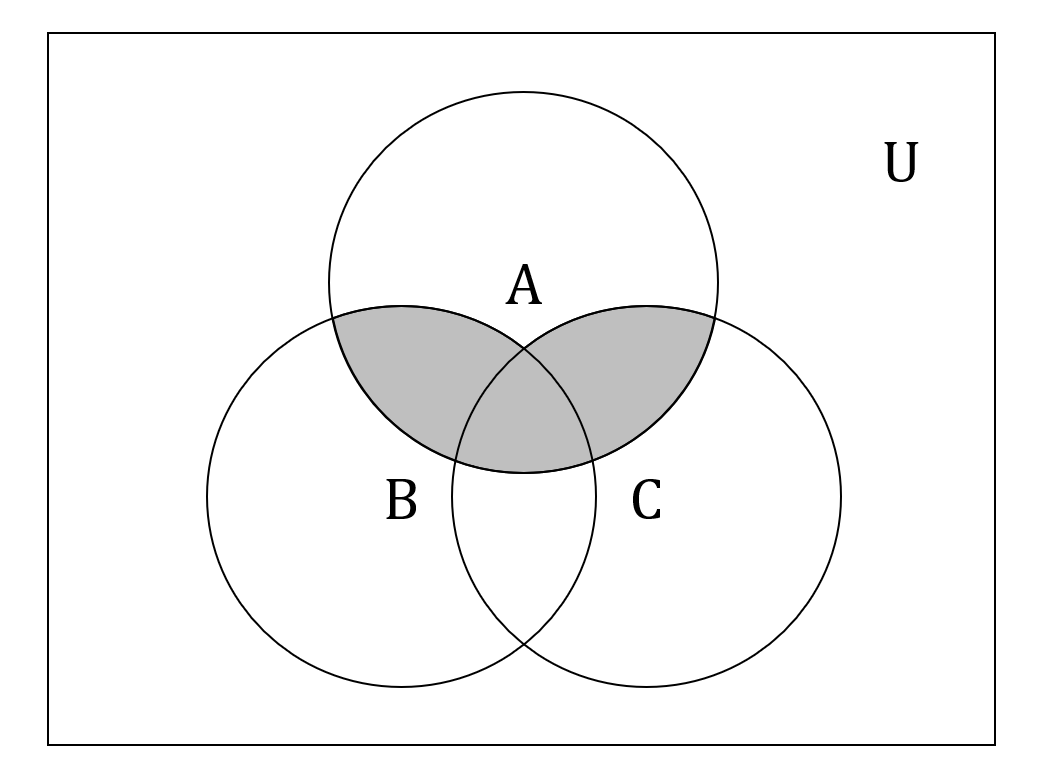
\includegraphics[width=0.35\linewidth]{VennA.png}
        \caption{Venn Diagram 2.1:16}
    \label{fig:2.2:26(a)}
\end{figure}
\begin{figure}[h]
 \centering
    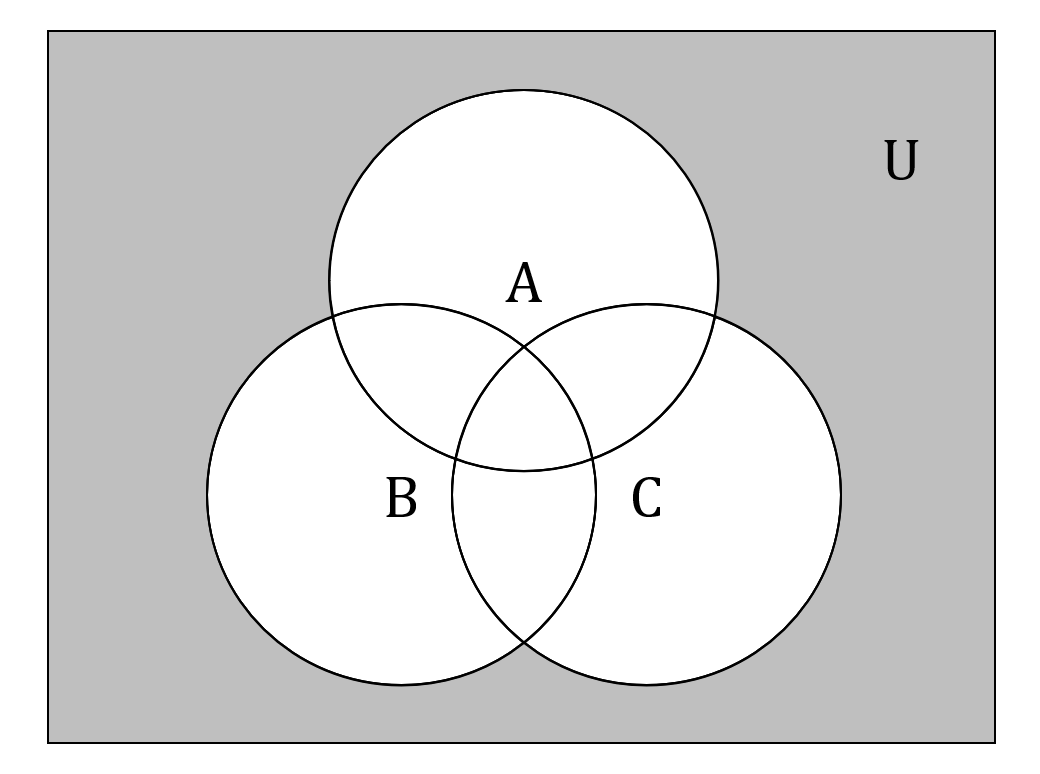
\includegraphics[width=0.35\linewidth]{VennB.png}
        \caption{Venn Diagram 2.1:16}
    \label{fig:2.2:26(b)}
\end{figure}
\begin{figure}[h]
 \centering
    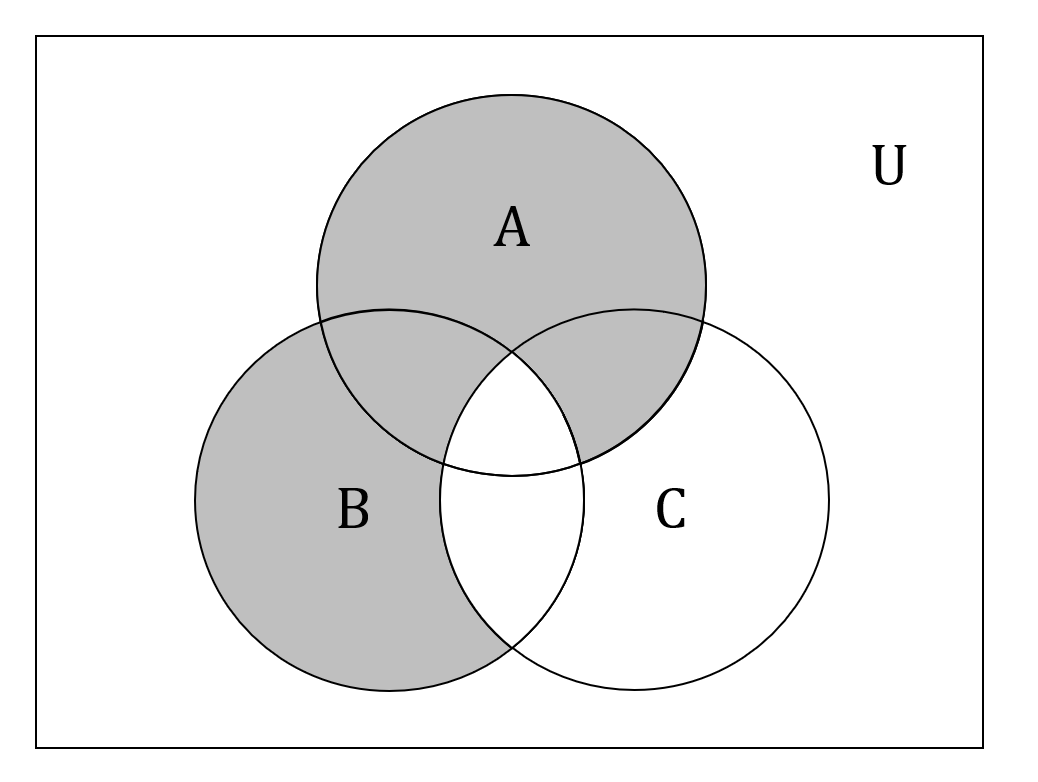
\includegraphics[width=0.33\linewidth]{VennD.png}
        \caption{Venn Diagram 2.1:16}
    \label{fig:2.2:26(c)}
\end{figure}
\end{document}
